\documentclass[a4paper,12pt]{article}
\usepackage[utf8]{inputenc}

%  Русский язык
\usepackage{multirow}
\usepackage{wrapfig}
\usepackage[T2A]{fontenc}			% кодировка
\usepackage[utf8]{inputenc}			% кодировка исходного текста
\usepackage[english,russian]{babel}	% локализация и переносы

\usepackage{indentfirst} %Красная строка
\usepackage[a4paper,top=1.3cm,bottom=2cm,left=1.5cm,right=1.5cm,marginparwidth=0.5cm]{geometry}
\usepackage[usenames]{color}
\usepackage{colortbl}
\usepackage{csvsimple}
\usepackage{siunitx}

\addto\captionsrussian{\def\refname{5   Список используемой литературы}}

% Заметки
\usepackage{todonotes}

% Математика
\usepackage{amsmath,amsfonts,amssymb,amsthm,mathtools} 
\usepackage{hyperref}

\renewcommand{\AA}{\ensuremath{\mathring{A}}}

\begin{document}
\def\figurename{Рисунок}
\begin{titlepage}

\begin{center}
    {\large МОСКОВСКИЙ ФИЗИКО-ТЕХНИЧЕСКИЙ ИНСТИТУТ (НАЦИОНАЛЬНЫЙ ИССЛЕДОВАТЕЛЬСКИЙ УНИВЕРСИТЕТ)}
\end{center}
\begin{center}
    {\largeФизтех-школа биологической и медицинской физики}
\end{center}

\vspace{1cm}
{\huge
\begin{center}
    {\bf Лабораторная работа по физической химии}\\
    \vspace{0.5cm}
    Электрокапиллярные явления
\end{center}
}

\vspace{4cm}
\begin{flushright}
{\LARGE Выполнили студенты группы Б06-103:\\ Кулешов Константин, Фитэль Алена \\}

\end{flushright}
\vspace{9cm}
\begin{center}
    Долгопрудный, 2023 г.
\end{center}
\end{titlepage}

\newpage
\newpage
\section{Введение}
\textbf{Цели работы}: Исследовать зависимость поверхностного натяжения от электрического потенциала на границе ртуть/раствор. Определить потенциал нулевого
заряда и ёмкость двойного электрического слоя на поверхности ртутного электрода в растворе. Оценить параметры плотной части ДЭС. Исследовать влияние природы электролита на потенциал нулевого заряда и
величину максимального натяжения.
\section{Теоретическое введение}
\subsection{Электрокапиллярные явления}
Суть электрокапиллярных явлений заключается в изменении межфазного натяжения на поверхности раздела в результате ее заряжения. При постоянном составе
электролита зависимость натяжения σ от разности потенциалов E определяется
(первым) уравнением Липпмана, максимальное натяжение соответствует так называемому потенциалу нулевого заряда:
\[
		q = -\Sigma(\frac{\partial\sigma}{\partial{E}})_{c_{i}}
	\]
Это уравнение следует из фундаментального уравнения Гиббса для изотермы
адсорбции ионов на границе электрод/раствор:
\[
		d\sigma = -qdE - \Sigma\Gamma_{i}d\mu_{i}
	\]
Так как $\mu_{i} = \mu^{0}_{i}+RT\ln c_{i}$, то уравнение Гиббса можно записать в виде:
\[
d\sigma = -qdE - RT\Sigma\Gamma_{i}d\ln c_{i}
\]
Из него также следует второе уравнение Липпмана для удельной емкости двойного электрического слоя:
\[
C = (\frac{\partial q}{\partial E})_{c_{i}} = -(\frac{\partial^{2}\sigma}{\partial E^{2}})_{c_{i}}
\]
В рамках модели Гельмгольца емкость двойного электрического слоя не зависит
от разности потенциала, поэтому электрокапиллярная кривая имеет вид параболы:
\[
\sigma - \sigma_{0} = -C\frac{(E-E_{0})^{2}}{2}
\]
где $E_{0}$ – потенциал нулевого заряда.
Если на поверхность ртути или другого металла, находящегося под слоем водного раствора, нанести каплю неполярной органической жидкости, нерастворимой
в воде (например, декана), то на трехфазной границе устанавливается равновесие
сил поверхностного натяжения (см. рис. 1) в соответствии с уравнением Юнга:
\begin{equation}
\sigma_{Hg/solution} = \sigma_{Hg/decan} +\sigma_{decan/H_{2}O}\cdot\cos\theta,
\end{equation}

При создании разности потенциалов между ртутью и водным раствором на этой межфазной границе возникает двойной электрический слой и межфазное натяжение σ31 меняется в соответствии с уравнением Липпмана при изменении разности
потенциалов. На других межфазных границах натяжение практически не меняется. Это и позволяет исследовать изменение поверхностного натяжения на границе
раздела ртутный электрод-раствор электролита в зависимости от потенциала электрода с помощью измерения краевого угла смачивания органической жидкости $\theta$.

\begin{figure}[h!]
    \centering
    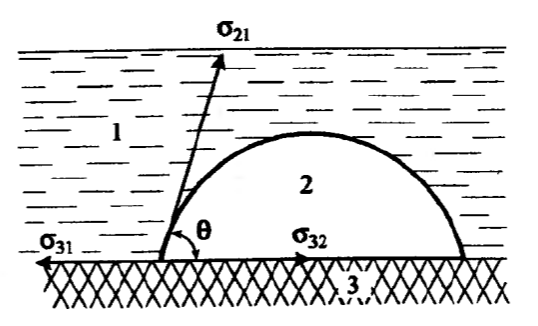
\includegraphics[width=7cm]{1.png}
    \caption{Силы, действующие на границе раздела фаз: металл (3) – водный раствор электролита (1) органическая жидкость (2)}
    \label{fig:vac}
\end{figure}
\subsection{Поляризуемые и неполяризуемые электроды}
Поляризацией электрода называют изменение потенциала электрода под действием электрического тока. Электрический ток может быть связан с протеканием
окислительно-восстановительного процесса (фарадеевский ток) на электроде, либо с заряжением двойного электрического слоя (ток заряжения). Очевидно, что
обе эти характеристики зависят от величины потенциала электрода, но в зависимости от природы электродов и состава электролитов изменение потенциала может в большей степени приводить к изменению заряда или протекающего тока
электрохимической реакции. Для наглядного понимания этих различий необходимо ознакомится с простейшей эквивалентной электрической схемой электрода, так
называемой схемой Эршлера-Рэндлса.

\begin{figure}[h!]
    \centering
    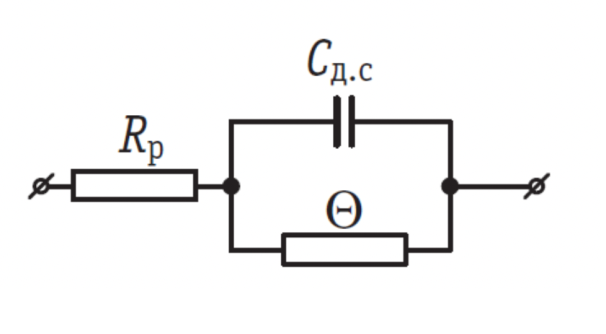
\includegraphics[width=7cm]{2.png}
    \caption{Силы, действующие на границе раздела фаз: металл (3) – водный раствор электролита (1) органическая жидкость (2)}
    \label{fig:vac}
\end{figure}

Величина фарадеевского сопротивления Θ обусловлена тем, что для протекания любого электрохимического процесса на электроде существует определенный
энергетический барьер. Для протекания заметного тока и преодоления этого барьера необходимо прикладывать к электроду определенную величину так называемого перенапряжения. Если величина сопротивления Θ велика, протекание реакции разряда затруднено и при незначительных приложенных напряжениях электрод ведет себя как конденсатор. Все приложенное напряжение идет на заряжение
емкости двойного электрического слоя. В этом идеальном случае эквивалентная
электрическая схема электрода представляет собой конденсатор C.. последовательно соединенный с резистором R. На идеально поляризуемых электродах изучаются
электрокапиллярные явления, описываемые уравнением Липпмана.

Другой крайний случай – идеально неполяризуемые электроды, электроды с
очень низким сопротивлением реакции разряда Θ. Благодаря этому они всегда
находятся в равновесии с продуктами электрохимической реакции и зарядить их
поверхность с помощью внешнего источника напряжения практически невозможно.

Типичными представителями обратимых идеально неполяризуемых электродов, обладающих высокой плотностью тока обмена, являются все электроды сравнения.

\subsection{Трехэлектродная электрохимическая ячейка}

Для проведения электрохимических измерений при контролируемом потенциале
электрода необходимо иметь способ достоверно фиксировать его величину и изменение. Наиболее известным методом решения этой задачи является использование
трехэлектродной схемы. Она включает в себя рабочий (исследуемый) электрод РЭ,
вспомогательный электрод ВЭ и электрод сравнения ЭС. В простейшем случае
при создании разности потенциалов между рабочим и вспомогательным электродом они оба заряжаются и, соответственно, часть общей разности потенциалов
падает в двойных электрических слоях вблизи их поверхности. В случае идеально
поляризуемого электрода других скачков напряжения не будет, но наличие двух
одновременно изменяемых компонент не позволит определить, какая часть общего
напряжения падает на рабочем электроде.
\begin{figure}[h!]
    \centering
    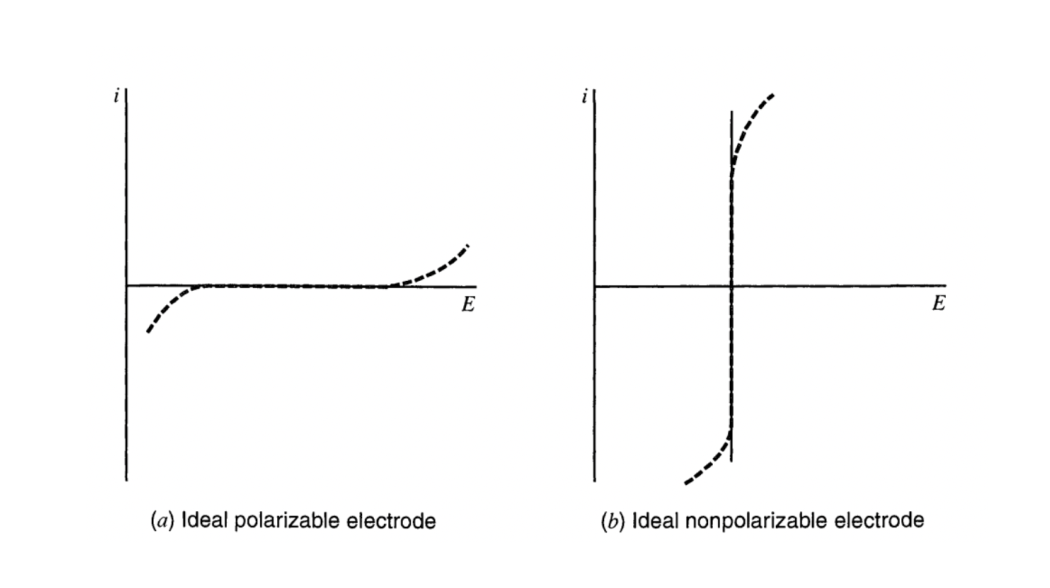
\includegraphics[width=7cm]{3.png}
    \caption{Кривые зависимости тока от потенциала для идеально поляризуемого (a) и идеально неполяризуемого (b) электродов.}
    \label{fig:vac}
\end{figure}


При протекании тока электрохимической реакции дополнительным неизвестным будет омическое падение напряжения
IR
цепи в растворе (линейный участок), и напряжение U на концах цепи равно:
\[
U = E_{0} + |\delta E_{\text{РЭ}}| + |\delta E_{\text{ВЭ}}|+ IR_{\text{цепи}}
\]
Так как при изменении тока, текущего в цепи, в правой части этого выражения
независимо изменяются три величины, то измеряемая в двухэлектродной схеме
величина U не может быть использована для характеристики состояния только
рабочего электрода. Двухэлектродная схема не позволяет определить величину
падения напряжения в двойном электрическом слое на исследуемом электроде при
ее варьировании от внешнего источника. Введение в измерительную схему третьего
электрода позволяет решить эту проблему.
Третий электрод – электрод сравнения по своей природе является идеально
обратимым электродом. Более того, он находится в высокоомной цепи высокоточного милливольтметра, поэтому через него практически не течет электрический
ток, что позволяет ему сохранять неизменным электрический потенциал. Этот потенциал, очевидно, определяется исключительно концентрацией потенциалопределяющих ионов около ЭС, которая не изменяется в ходе варьирования напряжения
между рабочим и вспомогательным электродами. Тем самым в цепи РЭ-ЭС с точностью до постоянного значения потенциала ЭС известно изменение потенциала
на рабочем электроде.
При измерении тока вспомогательный электрод не должен лимитировать измеряемую величину, поэтому площадь его поверхности должна заметно превышать
площадь рабочего электрода.
В электрохимии принято, что электрод называют катодом, если на нем протекает реакция восстановления, и анодом, если на нем протекает реакция окисления.
Рабочий электрод в трехэлектродной ячейке в зависимости от приложенного к
нему потенциала может являться как катодом, так и анодом. Электрод из металла
М в растворе соли того же металла является анодом, если его потенциал выше равновесного потенциала Eр системы Mz+/M. Соответственно, он является катодом
при E < E.

\begin{figure}[h!]
    \centering
    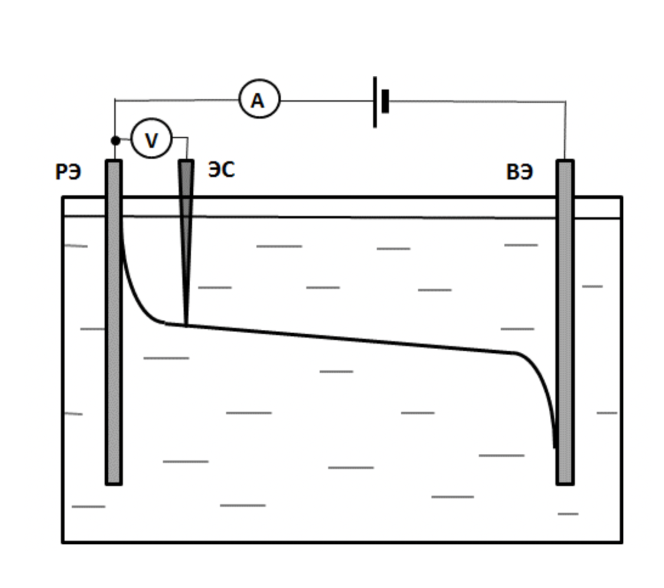
\includegraphics[width=7cm]{4.png}
    \caption{Схематическое представление трехэлектродной схемы измерений потенциала и тока. Обозначения на схеме: РЭ, ВЭ, СЭ – рабочий электрод, вспомогательный электрод и электрод сравнения, соответственно. Кривая между РЭ и ВЭ схематически показывает падение напряжения между этими электродами}
    \label{fig:vac}
\end{figure}

За положительный принят катодный ток, соответствующий прямому прохождению электрохимической реакции (восстановления) в стандартной ее записи:
\[
Ox + ne^{-} = Red
\]
Для задания и измерения потенциала и тока в электрохимической ячейке в
настоящее время вместо аккумулятора и делителя напряжения используют потенциостат.
\subsection{Многостадийность прохождения электрического тока}
Выше было показано, что деление электродов на поляризуемые и неполяризуемые, определяется величиной активационного барьера и скоростью кинетической
стадии переноса заряда на электроде. Таким образом, величина активационного
барьера электрохимической реакции определяет не только поляризуемость электрода, но и его вольтамперную характеристику при протекании тока. Любая электродная реакция, приводящая к протеканию электрического тока, как процесс,
происходящий на границе раздела фаз, сопряжена с протеканием нескольких последовательных стадий: массоперенос вещества из раствора к поверхности электрода, адсорбцию его на поверхности и собственно разряд - электрохимическую
реакцию переноса заряда на электрод. После прохождения реакции продукты также проходят аналогичные стадии для выделения в раствор. Скорость обратного
процесса определяется уже доставкой и реакцией этих продуктов на электроде.
Очевидно, как при любых последовательных реакциях, самая медленная стадия
будет определять общую скорость процесса, в данном случае – величину тока. Очевидно, что при низкой электропроводности раствора величина тока будет линейно
расти с напряжением в соответствии с законом Ома. Для элиминирования этого
процесса и изучения механизма других стадий протекания тока в систему вводят
повышенную концентрацию индифферентного электролита.

\section{Ход работы и обработка результатов}

\subsection{Исследование электрокапиллярной кривой ртути}
Исследование электрокапиллярной кривой на ртути проводится в данной работе с
помощью измерения краевого угла смачивания декана на поверхности ртути в
водном растворе 0.1 M NaF.

\begin{figure}[h!]
    \centering
    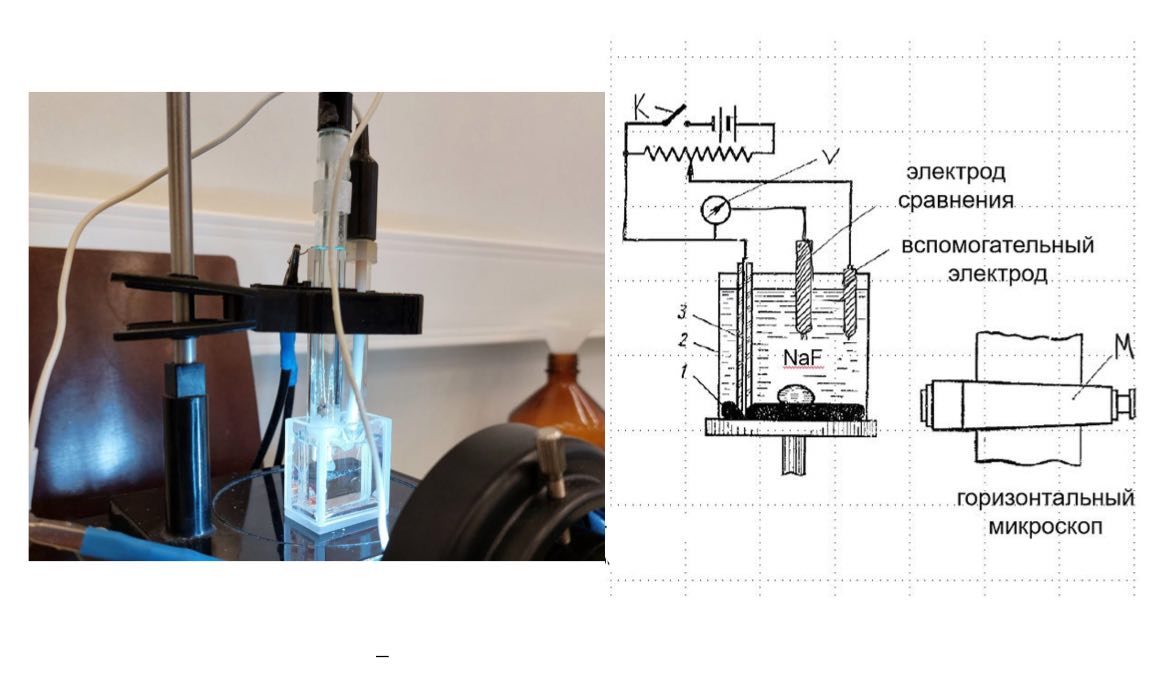
\includegraphics[width = 0.8\textwidth]{2022-12-29 02.14.12.jpg}
    \caption{Экспериментальная установка.}
    \label{fig:no_int}
\end{figure}\\

\subsubsection{Измерение краевого угла смачивания}

\begin{enumerate}

\item Подключим электроды к потенциостату по трёхэлектродной схеме:
контакты “Comp” и “Work” (+) потенциостата соединены и подключены к проволоке, погруженной в каплю ртути; контакт “Counter” (–) потенциостата подключён
к Pt противоэлектроду; контакт “Ref” (–) потенциостата подключён к хлорсеребрянному электроду сравнения.
Нанесем каплю декана объёмом 5 мкл на поверхность ртути. Варьированием
потенциала от -1300 мВ до 300 мВ относительно хлосеребряного электрода в циклическом режиме со скоростью развертки 50 мВ/c проведем тренировку капли.

\item Произведем измерения краевого угла смачивания от величины потенциала ртутного электрода в диапазоне от 3-- до -1300 мВ относительно хлорсеребряного электрода. Полученные фотографии капли декана с помощью программы ImageJ аппроксимируем окружностями и эллипсами для определения краевых углов смачивания. На основе результатов измерения краевого угла $\Theta(E)$ рассчитаем значение поверхностного натяжения границы ртуть/раствор по формуле (1). Табличные значения поверхносного натяжения на границах ртуть/декан и декан/вода, используемые для вычислений: $\sigma_{Hg/decan} = 375 \text{ мН/м}$, $\sigma_{decan/H_{2}O} = 51 \text{ мН/м}$ (\cite{1}). Полученные значения приведем в Таблице 1.

\begin{table}[h!]
\centering{%
\begin{tabular}{|r|r|r|
>{\columncolor[HTML]{FFFFFF}}r |r|}
\hline
\multicolumn{1}{|l|}{\textbf{E, мВ}} & \multicolumn{1}{l|}{\textbf{cos(\pi-\theta_{e})}} & \multicolumn{1}{l|}{\textbf{$\sigma_{e}$, мН/м}} & \multicolumn{1}{l|}{\cellcolor[HTML]{FFFFFF}\textbf{cos(\pi-\theta_{r})}} & \multicolumn{1}{l|}{\textbf{$\sigma_{r}$, мН/м}} \\ \hline
\multicolumn{1}{|l|}{-1298} & -0,606 & 344,07 & -0,561 & 346,38 \\ \hline
-1201 & -0,244 & 362,53 & -0,241 & 362,71 \\ \hline
-1100 & 0,221 & 386,25 & 0,256 & 388,06 \\ \hline
-1001 & 0,627 & 406,97 & 0,664 & 408,88 \\ \hline
-899 & 0,776 & 414,59 & 0,775 & 414,53 \\ \hline
-801 & 0,836 & 417,63 & 0,829 & 417,29 \\ \hline
-701 & 0,904 & 421,11 & 0,883 & 420,04 \\ \hline
-598 & 0,933 & 422,58 & 0,925 & 422,16 \\ \hline
-500 & 0,947 & 423,31 & 0,937 & 422,77 \\ \hline
-400 & 0,953 & 423,62 & 0,944 & 423,14 \\ \hline
-302 & 0,933 & 422,58 & 0,925 & 422,16 \\ \hline
-201 & 0,914 & 421,6 & 0,905 & 421,15 \\ \hline
-100 & 0,856 & 418,68 & 0,84 & 417,83 \\ \hline
1 & 0,776 & 414,59 & 0,764 & 413,97 \\ \hline
103 & 0,702 & 410,82 & 0,651 & 408,21 \\ \hline
200 & 0,64 & 407,66 & 0,571 & 404,13 \\ \hline
295 & 0,524 & 401,75 & 0,444 & 397,62 \\ \hline
\end{tabular}%
}
\caption{ Аппроксимация кругом и эллипсом электрокапиллярной кривой.
}
\label{tab:my-table}
\end{table}



\item Построим зависимость $\sigma_{Hg/solution}(E)$ по полученным данным (Рисунок 6). Аппроксимируем полученныю зависимость полиномом второй степени, найдем значения потенциала нулевого заряда относительно хлорсеребряного электрода
и величину поверхностного натяжения ртуть/раствор при этом $E$: 

\[
\sigma_{Hg/solution} = \sigma_{Hg/decane} + \sigma_{decane/H_{2}0}\cdot cos\theta
\]

\begin{figure}[h!]
    \centering
    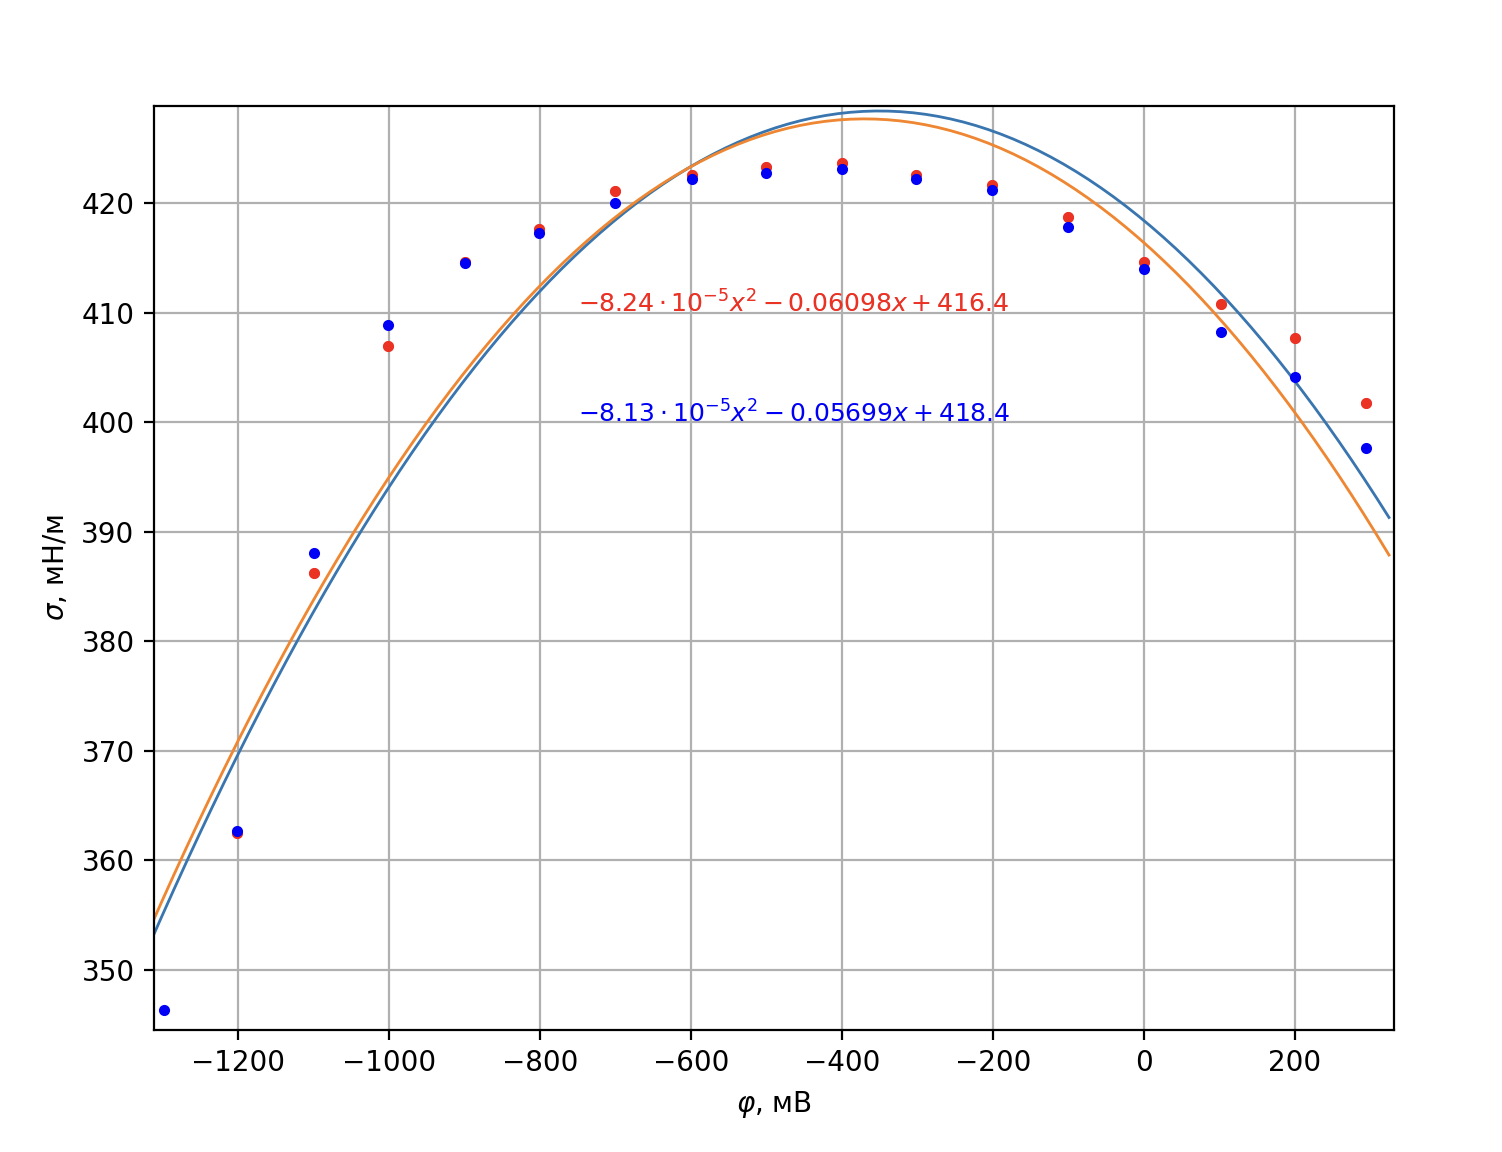
\includegraphics[width = 0.8\textwidth]{2.11.png}
    \caption{Электрокапиллярные кривые для разных аппроксимаций (синяя кривая - окружность, красная - эллипс).}
    \label{fig:no_int}
\end{figure}\\

\end{enumerate}

\newpage

\subsubsection{Расчет характеристик ДЭС ртутного электрода.}
\begin{enumerate}

\item Определим значение понециала нулевого заряда ртутного электрода. Для этого возьмем производную от полученной при аппроксимации кривой и приравняем ее к нулю. Найдем величину поверхностного натяжения ртуть/раствор при этом $E$ (Через ";" даны аппроксимации через окружность и через эллипс):

\[
\frac{d\sigma}{dE} = -8.13\cdot10^{-5} E - 0.057 = 0 ; \frac{d\sigma}{dE} = -8.24\cdot10^{-5} E - 0.061 = 0\]
\[
E_{\text{п.н.з}} = -386.3 \text{ мВ} ; E_{\text{п.н.з}} = -381.3 \text{ мВ}
\]
\[
\sigma_{Hg/solution} = 428.5 \text{ мН/м} ; \sigma_{Hg/solution} = 428.0 \text{ мН/м}
\]


\item Табличное значение ПНЗ ртутного электрода в 0.1М NaF относительно каломельного электрода \cite{2}:
    \begin{equation*}
        \varphi_{Hg} - \varphi_{cal} = -474 \text{ мВ}
    \end{equation*}
    Значения потенциалов хлорсеребряного и каломельного электродов относительно водородного \cite{2}:
    \begin{equation*}
        \varphi_{AgCl} - \varphi_{H2} = 222.34mV, \varphi_{cal} - \varphi_{H2} = 243.8 \text{ мВ}
    \end{equation*}
    \begin{equation*}
        \varphi_{Hg} - \varphi_{AgCl} = \varphi_{Hg} - \varphi_{cal} + \varphi_{cal} - \varphi_{H2} + \varphi_{H2} - \varphi_{AgCl} = -474 + 243.8 - 222.34 = -452.5 \text{ мВ}
    \end{equation*}

\item Расчитаем величину емкости двойного электрического слоя согласно модели Гельмгольца (концентрация электролита достаточно большая (0.1 М), поэтому $C \approx C_{\text{Г}$):

 \begin{equation*}
    \sigma = \sigma_{pnz} - \frac{C}{2}(\varphi - \varphi_{pnz})^2
    \end{equation*}
    \begin{equation*}
        \frac{d^2\sigma}{d\varphi^2} = \frac{d}{d\varphi} (-C(\varphi - \varphi_{pnz}) = -C
    \end{equation*}
    \begin{equation*}
        C = - \frac{d^2\sigma}{d\varphi^2} =  16 \frac{\text{мкФ}}{\text{см}^2} ; C = - \frac{d^2\sigma}{d\varphi^2} =  16 \frac{\text{мкФ}}{\text{см}^2}
    \end{equation*}

\item Оценим толщину ДЭС. В моделе Гельмгольца: $C_{\text{г}} = \frac{\epsilon \epsilon_0}{d}$, где d - искомая толщина ДЭС, $\epsilon_{0} = 8.855\cdot10^{-12} \frac{\text{Ф}}{\text{м}}$ - диэлектрическая постоянная, $\epsilon$ - диэлектрическая проницаемость воды. Диэлектрическая проницаемость "свободной" воды $\epsilon \approx 80$. Однако в данном случае молекулы воды поляризуются под действием внешнего электрического поля, в результате чего итоговая диэлектрическая проницаемость среды падает. Будем считать, что $\epsilon = 6 $. Тогда получим:
\[
 d = \frac{\epsilon \epsilon_0}{C} = \frac{8.855 \cdot 10^{-12} \cdot 6}{16} \frac{\text{Ф}}{\text{м}} \frac{\text{см}^{2}}{\text{мкФ}} = 3,32 \cdot 10^{-10} \text{м} = 3,32  \AA ;
\]

\end{enumerate}

\subsubsection{Сравнение результатов с моделями Гельмгольца и Гуи-Чапмена}

\begin{enumerate}
\item \textbf{Модель Гельмгольца}. В модели Гельмгольца толщина ДЭС - это радиус гидратированного иона. Оценим его с помощью модели Стокса:
\begin{center}
    $D = BkT$ \hspace{1cm} $B = \frac{1}{6 \pi r \eta}$ \hspace{1cm} $r = \frac{kT}{6 \pi D \eta}$
\end{center}

Справочные данные(\cite{2}):
\begin{center}
        $D_{Na^{+}} = 1.338\cdot 10^{-9} \frac{\text{м}^{2}}{\text{с}}$ \hspace{1cm} $D_{F^{-}} = 1.480\cdot 10^{-9} \frac{\text{м}^{2}}{\text{с}}$
    \end{center}
Тогда значения радиусов гидратированных ионов:
\begin{center}
    $r_{Na^{+}} = 1.832\AA$ \hspace{1cm} $r_{F^{-}} = 1.656\AA$
\end{center}
Данные значения гидратированного радиуса ионов меньше полученной оценки d. Это могло произойти из-за того, что диэлектрическая проницаемость воды в плотном слое не равна 6. Диэлектрическая проницаемость воды в плотном слое по нашим данным: 
\begin{equation*}
    d \sim \epsilon \Rightarrow \frac{\epsilon}{6} = \frac{r}{d} \Rightarrow \epsilon = 3.1
\end{equation*}

\item \textbf{Модель Гуи-Чапмена}. Оценим ёмкость диффузного слоя при потенциале нулевого заряда, используя модель Гуи-Чапмена: 
\begin{center}
    $\varphi = 0$ \hspace{1cm} $c_0 = 0.1 \text{ М}$ \hspace{1cm} $z = 1$
\end{center}

\[
C_{\text{ГЧ}} = \sqrt{\frac{2\epsilon \epsilon_0 F^2 c_{0}z^{2}}{RT}}\cosh(\frac{zF\varphi}{2RT}) =  \sqrt{\frac{2\epsilon \epsilon_0 F^2 c_{0}}{RT}} = 63.2 \frac{\text{мкФ}}{\text{см}^{2}}
\]
\item \textbf{Модель Штерна}. Оценим значение ёмкости ДЭС по модели Штерна, являющейся обобщением модели Гельмгольца и Гуи-Чапмена:
\begin{equation*}
    \frac{1}{C_{\Gamma}} = \frac{1}{C} - \frac{1}{C_d} \Rightarrow C = 21.4 \frac{\text{мкФ}}{\text{см}^2} \Rightarrow d = 2.5 \AA
\end{equation*}

\end{enumerate}

\subsection{Исследование поляризуемости ртутного электрода в растворе NaF}
Данная серия измерений проводится в растворе 0,1 М NaF.
\begin{enumerate}
    \item Проведем измерение циклической вольт-амперной характеристики для Hg
рабочего электрода (от –2100 до 300 мВ относительно хлорсеребряного электрода
сравнения при скорости развертки –50 мВ/с, старт с 0 мВ относительно текущего
потенциала разрыва цепи).
При низких потенциалах рабочего электрода на вспомогательном наблюдается
выделение газа - предположительно, водорода.
Потенциал разрыва цепи меняется со временем - порядка 25 мВ за первую
минуту.
Вид вольт-амперной характеристики (Рис. 7) показывает, что ртутный электрод
можно считать идеально поляризуемым в диапазоне от -1000 мВ до -100 мВ. 
\begin{figure}[h!]
    \centering
    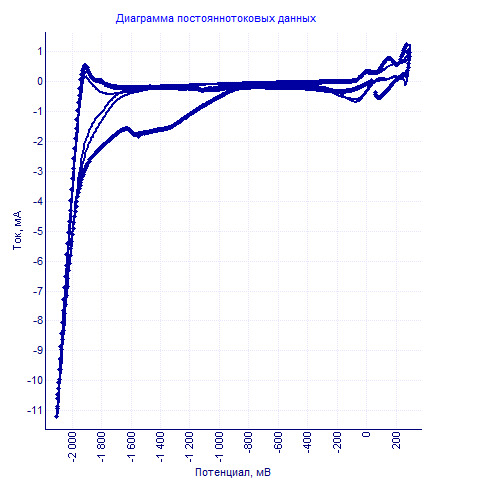
\includegraphics[width=7cm]{2.1.jpg}
    \caption{ЦВАХ Hg электрода}
    \label{fig:vac}
\end{figure}
\item Проведем обработку рабочего электрода - выдержим его в течение 3 минут при потенциале –2300 мВ относительно хлорсеребряного электрода сравнения. После обработки потенциал разрыва цепи падает и становится равным $-2016$ мВ, и теперь медленно меняется с течением времени. Это связано с тем, ионы $Na^{+}$ притягиваются к отрицательно заряженной поверхности ртути и образуется амальгама:
\[
Na^+ + nHg + e^- = Na\cdot Hg_{n}
\]
\item Произведем измерение циклической вольт-амперной характеристики для обработанного Hg рабочего электрода (от –2200 до –1800 мВ относительно хлорсеребряного
электрода сравнения при скорости развертки –50 мВ/с, старт с 0 мВ относительно текущего потенциала разрыва цепи). Из графика (Рис. 8) видно, что электрод
потерял свойство поляризуемости.
\begin{figure}[h!]
    \centering
    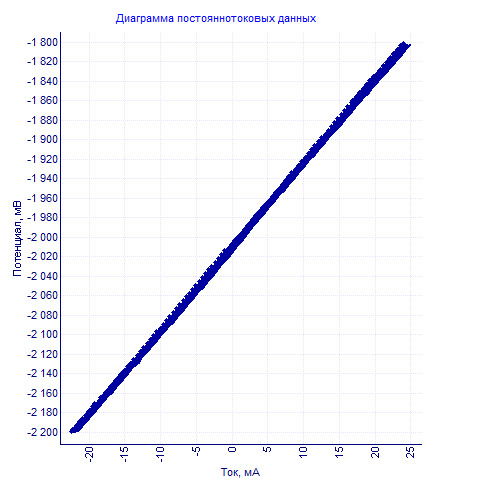
\includegraphics[width=8cm]{2.2.jpg}
    \caption{ЦВАХ Hg электрода после обработки (напряжение: от –2200 до –1800 мВ относительно хлорсеребряного электрода сравнения)}
    \label{fig:vac}
\end{figure}

\item Произведем измерение циклической вольт-амперной характеристики для обработанного
Hg рабочего электрода (от –2100 до 300 мВ относительно хлорсеребряного
электрода сравнения при скорости развертки –50 мВ/с, старт с 0 мВ относительно
текущего потенциала разрыва цепи) (Рис. 9). 
В процессе проведения эксперимента было зафиксировано бурное выделение газа, что может свидетельствовать о переходе ионов натрия в водный раствор с выделением водорода, согласно уравнению реакции:
\[
Na + H_{2}O = NaOH + \frac{1}{2} H_{2}
\]

\begin{figure}[h!]
    \centering
    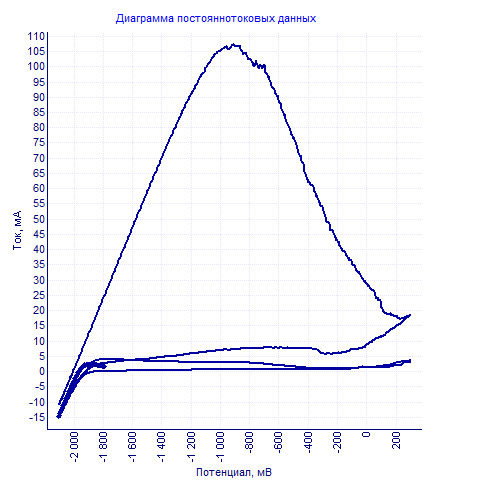
\includegraphics[width=8cm]{2.3.jpg}
    \caption{ЦВАХ Hg электрода после обработки (напряжение: от –2100 до 300 мВ относительно хлорсеребряного электрода сравнения) }
    \label{fig:vac}
\end{figure}

\end{enumerate}

\newpage
\section{Обсуждение результатов и вывод}
\begin{itemize}
    \item В ходе работы была построена электрокапиллярная кривая границы раздела ртуть-раствор электролита.
    \item Получена оценка потенциала нулевого заряда ртутного электрода в 0.1M NaF относительно хлорсеребрянного электрода: 
    \begin{equation*}
       E_{\text{п.н.з}}}= -386.3 \text{ мВ} ; E_{\text{п.н.з}}= -381.3 \text{ мВ}
    \end{equation*}
    
   Полученные резульаты близки к справочному: $E_{\text{п.н.з}} = -452.5 \text{ мВ}$.
    \item Рассчитаны параметры двойного электрического слоя  по моделям Штерна, Гельмгольца и Гуи-Чапмана:

\[C = 21.4\;\frac{\text{мкФ}}{\text{см$^2$}},\;\; C_{\text{Г}} = 16\;\frac{\text{мкФ}}{\text{см$^2$}},\;\; C_{\text{ГЧ}} = 63.2\;\frac{\text{мкФ}}{\text{см$^2$}}\]

\[d_{\text{Г}} = 3.32\buildrel _{\circ} \over {\mathrm{A}} ,  d = 2.5\buildrel _{\circ} \over {\mathrm{A}}\]

    \item Также построена ЦВАХ ртутного электрода до обработки и после обработки потенциалом -2300 мВ. До обработки потенциалом электрод являлся поляризуемым электродом, а после обработки стал неполяризуемым в некотором диапазоне потенциала, однако после подачи высокого потенциала электрод вернулся в поляризованное состояние.

\end{itemize}


%Из получившегося графика видно, что максимум электрокапилллярной кривой,построенный по точкам вдалеке от ПНЗ больше, чем максимум кривой, построенной по всем точкам. Этот эффект можно объяснить адсорбцией на поверхности ртути органических веществ (скорее всего примесей в декане). Действительно, органические вещества хорошо адсорбируются из полярного раствора (т.к. они неполярные). Но при больших потенциалах ионы так сильно притягиваются к поверхности, что вытесняют органические вещества. Т.о. вдали от ПНЗ нет адсорбированных органических веществ, поэтому будем рассматривать эти точки. Однако, если делать аппроксимацию по крайним точкам, то значение поверхностного натяжения превосходит табличное для границы ртуть - вода. Расчитаем значение пнз для параболы, построенной по всем точкам.%














\newpage
\addcontentsline{toc}{section}{Список используемой литературы}
\begin{thebibliography}{}
    \bibitem{1}  Кафедра общей химии МФТИ -  "Электрокапиллярные явления, свойства электродов"
    \bibitem{2}  Сухотин A.М., 1981 г.  -  "Справочник по электрохимии"
\end{thebibliography}


\end{document}

